\documentclass[12pt,a4paper]{article}
\usepackage[utf8]{inputenc}
\usepackage[T1]{fontenc}
\usepackage[french]{babel}
\usepackage{graphicx}
\usepackage{hyperref}
\usepackage{geometry}
\usepackage{xcolor}
\usepackage{listings}
\usepackage{titlesec}
\usepackage{float}
\usepackage{tikz}
\usetikzlibrary{shapes.geometric, arrows.meta, positioning}
\usepackage{booktabs}

\geometry{top=2.5cm, bottom=2.5cm, left=2.5cm, right=2.5cm}
\graphicspath{{screenshots/}}

\lstset{
    language=Python,
    basicstyle=\ttfamily\footnotesize,
    keywordstyle=\color{blue}\bfseries,
    stringstyle=\color{green!50!black},
    commentstyle=\color{gray}\itshape,
    showstringspaces=false,
    frame=single,
    breaklines=true,
    backgroundcolor=\color{black!5},
    literate={é}{{\'{e}}}1 {è}{{\`{e}}}1 {ê}{{\^{e}}}1 {à}{{\`{a}}}1 {â}{{\^{a}}}1 {ô}{{\^{o}}}1 {û}{{\^{u}}}1 {ç}{{\c{c}}}1 {É}{{\'{E}}}1
}

\begin{document}

\begin{titlepage}
    \centering
    \vspace*{1cm}
    
    {\Large \textbf{Universit\'e Hassan II de Casablanca}} \\
    {\Large \textbf{ENSET Mohammedia}} \\
    \vspace{0.5cm}
    {\large \textbf{Master SDIA (Smart Distributed and Intelligent Applications)}} \\
    {\large \textbf{Parcours : SMA et IAD}} \\
    
    \vspace{3cm}
    
    \rule{\linewidth}{0.5mm} \\
    \vspace{0.5cm}
    {\huge \textbf{PROJET DE FIN DE MODULE}} \\
    \vspace{0.3cm}
    {\Large \textit{Ecosyst\`eme Multi-Agent : Architecte Mat\'eriel PC}} \\
    \rule{\linewidth}{0.5mm}
    
    \vspace{3cm}
    
    \begin{flushleft}
        \large
        \textbf{R\'ealis\'e par :} \\
        Marouane MAHBOUB \\
        Abderahim FARAHI \\
    \end{flushleft}
    
    \vspace{1cm}
    
    \begin{flushright}
        \large
        \textbf{Encadr\'e par :} \\
        Pr. Sara RETAL
    \end{flushright}
    
    \vfill
    
    \centering
    \textbf{Code Source :} \\
    \url{https://github.com/marouane-m7b/ENSET_PFM_Agent_Building_PC}
    
    \vspace{1cm}
    {\large \today}
\end{titlepage}

\tableofcontents
\newpage

\section{Introduction et Choix du Sujet}
Pour ce projet de fin de module, nous avons choisi de d\'evelopper un \textbf{Architecte Mat\'eriel PC (Custom PC Builder)}. Le choix de ce sujet n'est pas fortuit : l'assemblage d'un ordinateur est un probl\`eme complexe d'ing\'enierie et de satisfaction de contraintes. 

\textbf{Pourquoi ce sujet ?}
\begin{itemize}
    \item \textbf{Pertinence pour le Multi-Agent :} Contrairement \`a un chatbot classique, construire un PC n\'ecessite plusieurs expertises distinctes : planifier un budget, v\'erifier la compatibilit\'e physique (Sockets, DDR4 vs DDR5), et acheter au meilleur prix.
    \item \textbf{N\'ecessit\'e du RAG :} Le march\'e du hardware \'evolue chaque jour. Un grand mod\`ele de langage (LLM) seul proposerait des composants obsol\`etes ou hors stock. L'utilisation du RAG \'etait indispensable pour connecter l'agent \`a un inventaire local en temps r\'eel.
    \item \textbf{Besoin du Human-in-the-Loop :} L'achat de mat\'eriel co\^utant parfois des dizaines de milliers de dirhams, il est impensable de laisser l'IA finaliser une transaction sans l'approbation humaine finale.
\end{itemize}

\section{D\'etails d'Impl\'ementation (Technologies Utilis\'ees)}
Le code source de notre projet a \'et\'e structur\'e de mani\`ere modulaire autour des technologies de pointe de l'\'ecosyst\`eme IA :
\begin{itemize}
    \item \textbf{LangGraph :} Utilis\'e pour concevoir l'orchestrateur (StateGraph). Il maintient l'\'etat global (BuilderState) et permet d'interrompre l'ex\'ecution via interrupt\_before pour le Human-in-the-Loop.
    \item \textbf{Groq API (LLaMA 3.3 70B) :} Mod\`ele de langage utilis\'e pour l'analyse s\'emantique des requ\^etes (Agent Architecte) et la strat\'egie de s\'election (Agent Procurement). Choisi pour sa rapidit\'e d'inf\'erence.
    \item \textbf{ChromaDB + nomic-embed-text :} Base de donn\'ees vectorielle (RAG) aliment\'ee par les embeddings locaux d'Ollama. Nos 8 fichiers CSV d'inventaire (CPUs, GPUs, RAM, etc.) sont vectoris\'es et index\'es par cat\'egorie.
    \item \textbf{MySQL :} Base relationnelle pour la persistance de l'historique des conversations, des sessions et des d\'ecisions d'approbation.
    \item \textbf{Flask / Socket.IO :} Backend web temps r\'eel. Socket.IO \'emet des \'ev\'enements (agent\_status, approval\_needed, discord\_sent) pour synchroniser l'\'etat du workflow avec le frontend.
    \item \textbf{Discord Webhook :} Int\'egration pour envoyer automatiquement les builds approuv\'es vers un canal Discord d'\'equipe.
    \item \textbf{Pandas :} M\'ecanisme de fallback d\'eterministe si l'API Groq est indisponible (Rate Limits).
\end{itemize}

\section{Architecture du Syst\`eme Multi-Agent}
Dans le cadre de ce projet, nous avons d\'evelopp\'e un \'ecosyst\`eme intelligent capable de concevoir un ordinateur optimis\'e selon un budget pr\'ecis. Le flux de travail a \'et\'e d\'ecompos\'e s\'equentiellement avec une architecture modulaire avanc\'ee.

\begin{figure}[H]
\centering
\begin{tikzpicture}[node distance=1.8cm, auto,
    block/.style={rectangle, draw=blue!60, fill=blue!8, text width=2.8cm, text centered, rounded corners, minimum height=1.2cm, font=\small\bfseries},
    decision/.style={diamond, draw=orange!60, fill=orange!8, text width=1.6cm, text centered, aspect=2, font=\small\bfseries},
    io/.style={trapezium, draw=green!60, fill=green!8, trapezium left angle=70, trapezium right angle=110, text width=2cm, text centered, minimum height=1cm, font=\small\bfseries},
    arrow/.style={-Stealth, thick, draw=gray!70}]

    \node[io] (user) {Utilisateur};
    \node[block, right=of user] (arch) {Agent Architecte};
    \node[block, right=of arch] (proc) {Agent Procurement};
    \node[decision, below=1.5cm of proc] (hitl) {Approbation Humaine};
    \node[block, left=of hitl] (modify) {Modifier Build (3 Alternatives)};
    \node[io, below=1.5cm of hitl] (out) {Discord + Inventaire};

    \node[block, above=0.8cm of arch, fill=purple!8, draw=purple!60, text width=2.5cm] (rag) {RAG (ChromaDB)};
    \node[block, above=0.8cm of proc, fill=red!8, draw=red!60, text width=2.5cm] (llm) {Groq LLM};

    \draw[arrow] (user) -- node[above, font=\tiny]{Budget + Use Case} (arch);
    \draw[arrow] (arch) -- node[above, font=\tiny]{Requirements} (proc);
    \draw[arrow] (proc) -- node[right, font=\tiny]{Build} (hitl);
    \draw[arrow] (hitl) -- node[below, font=\tiny]{Rejet} (modify);
    \draw[arrow] (modify) |- node[near start, above, font=\tiny]{Swap} (proc);
    \draw[arrow] (hitl) -- node[right, font=\tiny]{Approuv\'e} (out);
    \draw[arrow, dashed] (rag) -- (arch);
    \draw[arrow, dashed] (rag) -- (proc);
    \draw[arrow, dashed] (llm) -- (arch);
    \draw[arrow, dashed] (llm) -- (proc);
\end{tikzpicture}
\caption{Architecture globale du syst\`eme multi-agent}
\label{fig:architecture}
\end{figure}

\subsection{Architecture Modulaire}
Le syst\`eme a \'et\'e structur\'e en modules ind\'ependants pour am\'eliorer la lisibilit\'e, la maintenabilit\'e et la r\'eutilisabilit\'e :

\begin{itemize}
    \item \textbf{Module agents/nodes.py :} Contient les impl\'ementations des agents individuels avec des classes sp\'ecialis\'ees (ArchitectAgent, ProcurementAgent)
    \item \textbf{Module human\_loop/ :} Syst\`eme complet de validation humaine avec gestion d'\'etat, interface utilisateur et int\'egration workflow
    \item \textbf{Module evaluation/ :} Framework d'\'evaluation et d'optimisation des prompts avec tests A/B
    \item \textbf{Module rag/ :} Syst\`eme de r\'ecup\'eration augment\'ee avec base vectorielle ChromaDB
\end{itemize}

\subsection{Agents Sp\'ecialis\'es}

\subsubsection{Agent Architecte (ArchitectAgent)}
Responsabilit\'es principales :
\begin{itemize}
    \item Analyse s\'emantique des requ\^etes utilisateur
    \item Extraction intelligente du budget avec patterns regex multiples
    \item Classification automatique des cas d'usage (gaming, IA/ML, bureautique, cr\'eation de contenu)
    \item D\'etermination du niveau de performance requis
\end{itemize}

\subsubsection{Agent Procurement (ProcurementAgent)}
Responsabilit\'es principales :
\begin{itemize}
    \item Interrogation de la base RAG avec filtrage cat\'egoriel
    \item Algorithme d'optimisation avec v\'erification de compatibilit\'e mat\'erielle
    \item G\'en\'eration de devis format\'es avec m\'etriques de performance
    \item Validation automatique des contraintes budg\'etaires
\end{itemize}

\subsubsection{Syst\`eme Human-in-the-Loop (HumanLoopWorkflow)}
Responsabilit\'es principales :
\begin{itemize}
    \item Gestionnaire d'approbation avec \'etats persistants
    \item Interface utilisateur modulaire avec composants Flask et SocketIO
    \item Int\'egration transparente avec LangGraph
    \item Historique et statistiques des d\'ecisions humaines
\end{itemize}

\subsection{Orchestration LangGraph}
L'orchestrateur utilise un StateGraph avec \'etat typ\'e (BuilderState) \'etendu pour supporter la gestion des m\'etadonn\'ees, le suivi des analyses et la persistance des composants.

\begin{lstlisting}[caption={D\'efinition du workflow LangGraph (graph.py)}]
class BuilderState(TypedDict):
    user_request: str
    architect_plan: str
    final_build_quote: str
    selected_components: dict
    total_price: int
    human_approval: str
    conversation_history: List[dict]

# Construction du graphe sequentiel
workflow = StateGraph(BuilderState)
workflow.add_node("architect", architect_node)
workflow.add_node("procurement", procurement_node)
workflow.add_node("human_approval", human_approval_node)

workflow.add_edge(START, "architect")
workflow.add_edge("architect", "procurement")
workflow.add_edge("procurement", "human_approval")
workflow.add_edge("human_approval", END)

# Compilation avec checkpoint et interruption
memory = MemorySaver()
agent_app = workflow.compile(
    checkpointer=memory,
    interrupt_before=["human_approval"]
)
\end{lstlisting}

La m\'ethode de collaboration choisie est \textbf{s\'equentielle} : chaque agent d\'epend de la sortie du pr\'ec\'edent. Ce choix se justifie car la s\'election de composants n\'ecessite d'abord une analyse des besoins (Architecte), puis une recherche optimis\'ee (Procurement), et enfin une validation humaine avant toute action irr\'eversible (mise \`a jour du stock et notification Discord).

\section{D\'efis Techniques et R\'esolution des Hallucinations}
Le d\'eveloppement de ce syst\`eme nous a confront\'es \`a plusieurs d\'efis d'ing\'enierie inh\'erents aux LLMs.

\subsection{Hallucinations de Satisfaction d'Objectif}
\textbf{Le Probl\`eme :} Initialement, l'Agent Procurement mentait sur les prix ou inventait des noms de composants inexistants (ex: "NVIDIA Radeon") dans le but math\'ematique de satisfaire parfaitement le budget impos\'e par l'utilisateur.

\textbf{La Solution :} Mise en place d'un m\'ecanisme de Chain-of-Thought (CoT) via une balise <thinking>. En for\c{c}ant l'agent \`a extraire les vrais prix du contexte RAG et \`a \'ecrire ses calculs d'addition \'etape par \'etape avant de g\'en\'erer le devis final, nous avons drastiquement r\'eduit les erreurs logiques et budg\'etaires.

\subsection{Limitations de la Recherche S\'emantique}
\textbf{Le Probl\`eme :} La base vectorielle ChromaDB filtrait parfois des composants critiques. La similitude s\'emantique \'echouait \`a comprendre qu'une requ\^ete pour du "High-End" correspondait concr\`etement \`a un "Core i7" ou un "Ryzen 9".

\textbf{La Solution :} Passage \`a une Recherche Cat\'egorielle Structur\'ee. Au lieu d'une seule recherche globale, le syst\`eme it\`ere sur un tableau de 8 cat\'egories (CPUs, GPUs, RAM, etc.) et effectue une r\'ecup\'eration sp\'ecifique pour chacune.

\begin{lstlisting}[caption={Recherche cat\'egorielle RAG}]
categories = ["CPUS", "GPUS", "MOTHERBOARDS", "RAM", 
              "STORAGE", "COOLERS", "PSUS", "CASES"]
full_context = []

for cat in categories:
    results = db.as_retriever(
        search_kwargs={"k": 2, "filter": {"category": cat}}
    ).invoke(plan)
    for doc in results:
        full_context.append(f"[CATEGORY: {cat}] {doc.page_content}")
\end{lstlisting}

\section{Evaluation et Optimisation des Prompts}

\subsection{Framework d'Evaluation Complet}
Nous avons d\'evelopp\'e un syst\`eme d'\'evaluation sophistiqu\'e pour optimiser les performances des prompts utilis\'es par nos agents.

\subsubsection{Tests A/B Automatis\'es}
Le framework impl\'emente une m\'ethodologie de tests A/B rigoureuse :
\begin{itemize}
    \item \textbf{4 Strat\'egies de Prompts :} Basic, Detailed, Structured, Context-Aware
    \item \textbf{6 Sc\'enarios de Test :} Gaming, Workstation, Office, AI/ML, Streaming, Budget contraint
    \item \textbf{M\'etriques Multiples :} Pr\'ecision, adh\'erence budg\'etaire, compatibilit\'e, temps de r\'eponse, satisfaction utilisateur
    \item \textbf{Analyse Statistique :} Moyenne, m\'ediane, \'ecart-type, intervalles de confiance
\end{itemize}

\subsubsection{M\'etriques de Performance}
Le syst\`eme \'evalue cinq dimensions critiques :
\begin{itemize}
    \item \textbf{Pr\'ecision d'Extraction :} Capacit\'e \`a extraire correctement le budget et les exigences
    \item \textbf{Adh\'erence Budg\'etaire :} Respect des contraintes financi\`eres (tol\'erance plus ou moins 10 pourcent)
    \item \textbf{Compatibilit\'e Mat\'erielle :} V\'erification des compatibilit\'es CPU-Motherboard, RAM-CPU
    \item \textbf{Temps de R\'eponse :} Performance temporelle des diff\'erentes strat\'egies
    \item \textbf{Satisfaction Utilisateur :} Score composite bas\'e sur les autres m\'etriques
\end{itemize}

\subsection{R\'esultats de l'Optimisation}
Les tests A/B ont montr\'e que la strat\'egie \textbf{Context-Aware} (D) offre les meilleurs r\'esultats avec un score global de 0.765, soit une am\'elioration de 41\% par rapport \`a la strat\'egie de base. C'est cette strat\'egie qui a \'et\'e retenue en production.

\section{Interface Utilisateur et Human-in-the-Loop}

\subsection{Interface Wizard Interactive}
L'interface utilisateur a \'et\'e con\c{c}ue comme un \textbf{wizard interactif} (et non un simple chatbot) compos\'e de cinq \'ecrans :

\begin{enumerate}
    \item \textbf{\'Ecran d'Accueil :} S\'election du cas d'usage (Gaming, IA/ML, Bureautique, D\'eveloppement, Cr\'eation de Contenu, G\'en\'eral) et configuration du budget via un slider interactif ou un champ de saisie directe (5\,000 -- 80\,000 MAD).
    \item \textbf{\'Ecran de Construction IA :} Visualisation en temps r\'eel du pipeline multi-agent (Architecte $\rightarrow$ Procurement $\rightarrow$ Approbation) avec barres de progression anim\'ees.
    \item \textbf{\'Ecran R\'ecapitulatif :} Affichage des 8 composants s\'electionn\'es par l'IA avec co\^ut total, pourcentage du budget utilis\'e, \'economies et statut de compatibilit\'e. Deux actions : \textit{Approuver et Envoyer \`a Discord} ou \textit{Modifier le Build}.
    \item \textbf{\'Ecran de Modification :} Permet de cliquer sur n'importe quel composant pour afficher \textbf{3 alternatives au prix le plus proche}, tout en respectant les contraintes de compatibilit\'e (Socket CPU $\leftrightarrow$ Motherboard, DDR4/DDR5 $\leftrightarrow$ RAM).
    \item \textbf{\'Ecran de R\'esultat :} Confirmation de l'approbation avec mise \`a jour de l'inventaire et notification Discord.
\end{enumerate}

\begin{figure}[H]
\centering

\includegraphics[width=0.85\textwidth]{welcome.png}
\caption{\'Ecran d'accueil : s\'election du cas d'usage parmi 6 cat\'egories}
\label{fig:welcome}
\end{figure}

\begin{figure}[H]
\centering
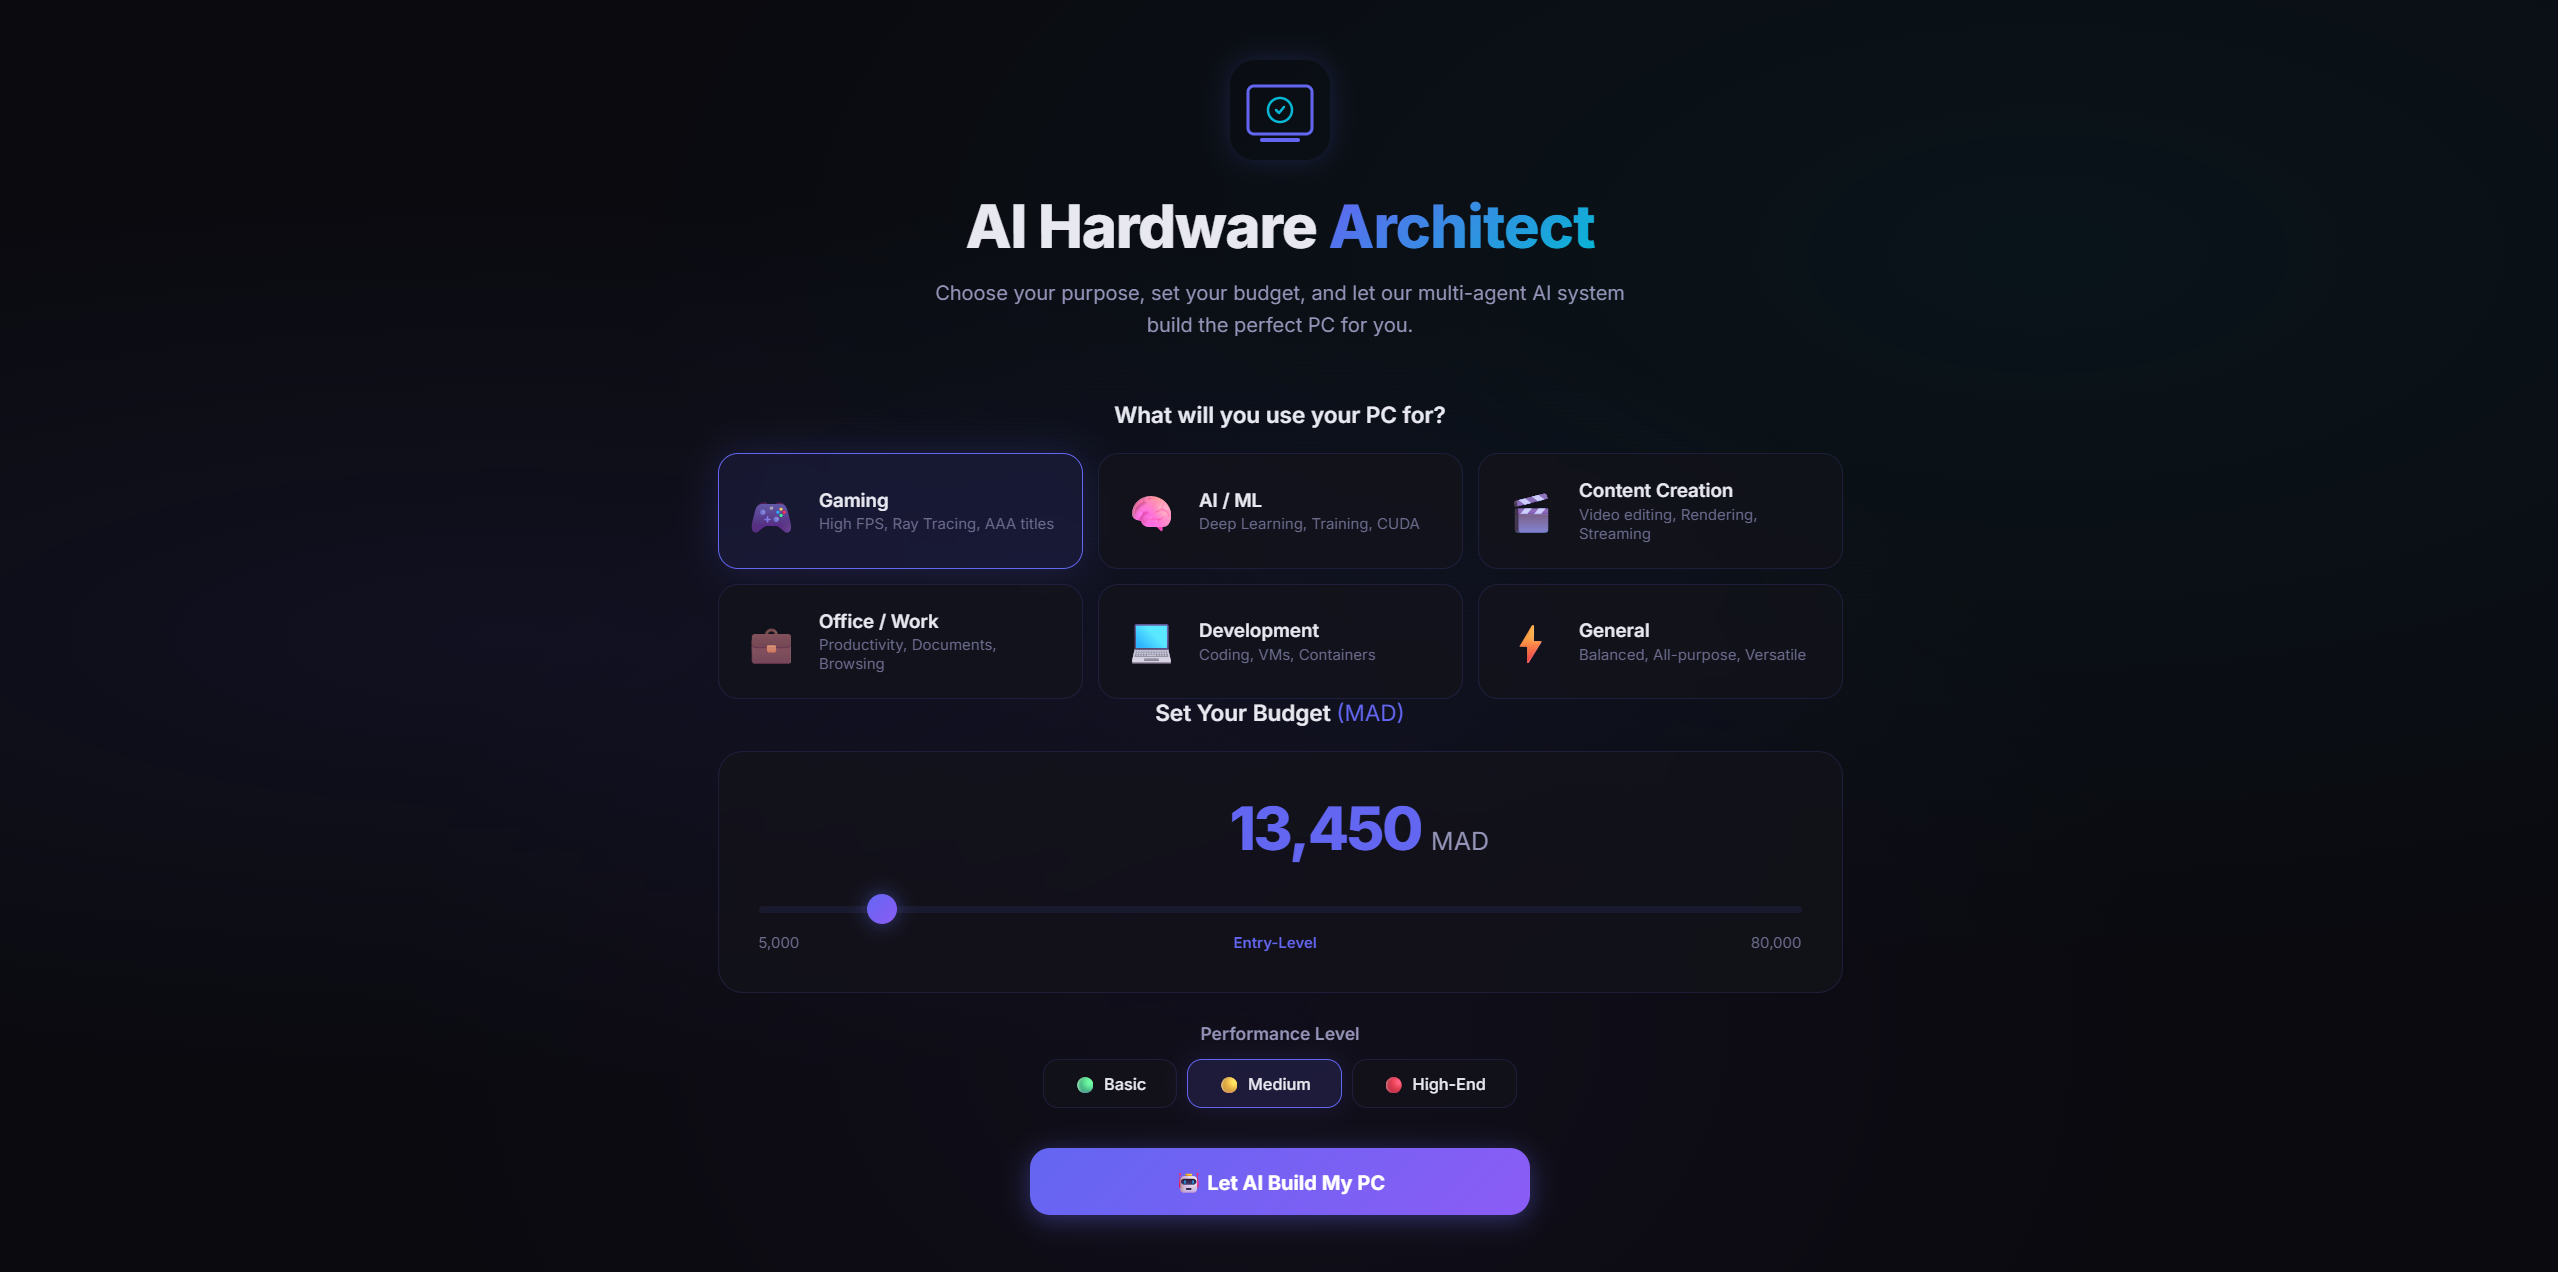
\includegraphics[width=0.85\textwidth]{budget.png}
\caption{Configuration du budget via slider interactif ou saisie directe, avec s\'election du niveau de performance}
\label{fig:budget}
\end{figure}

\begin{figure}[H]
\centering

\includegraphics[width=0.85\textwidth]{building.png}
\caption{\'Ecran de construction IA : visualisation en temps r\'eel du pipeline multi-agent}
\label{fig:building}
\end{figure}

\begin{figure}[H]
\centering
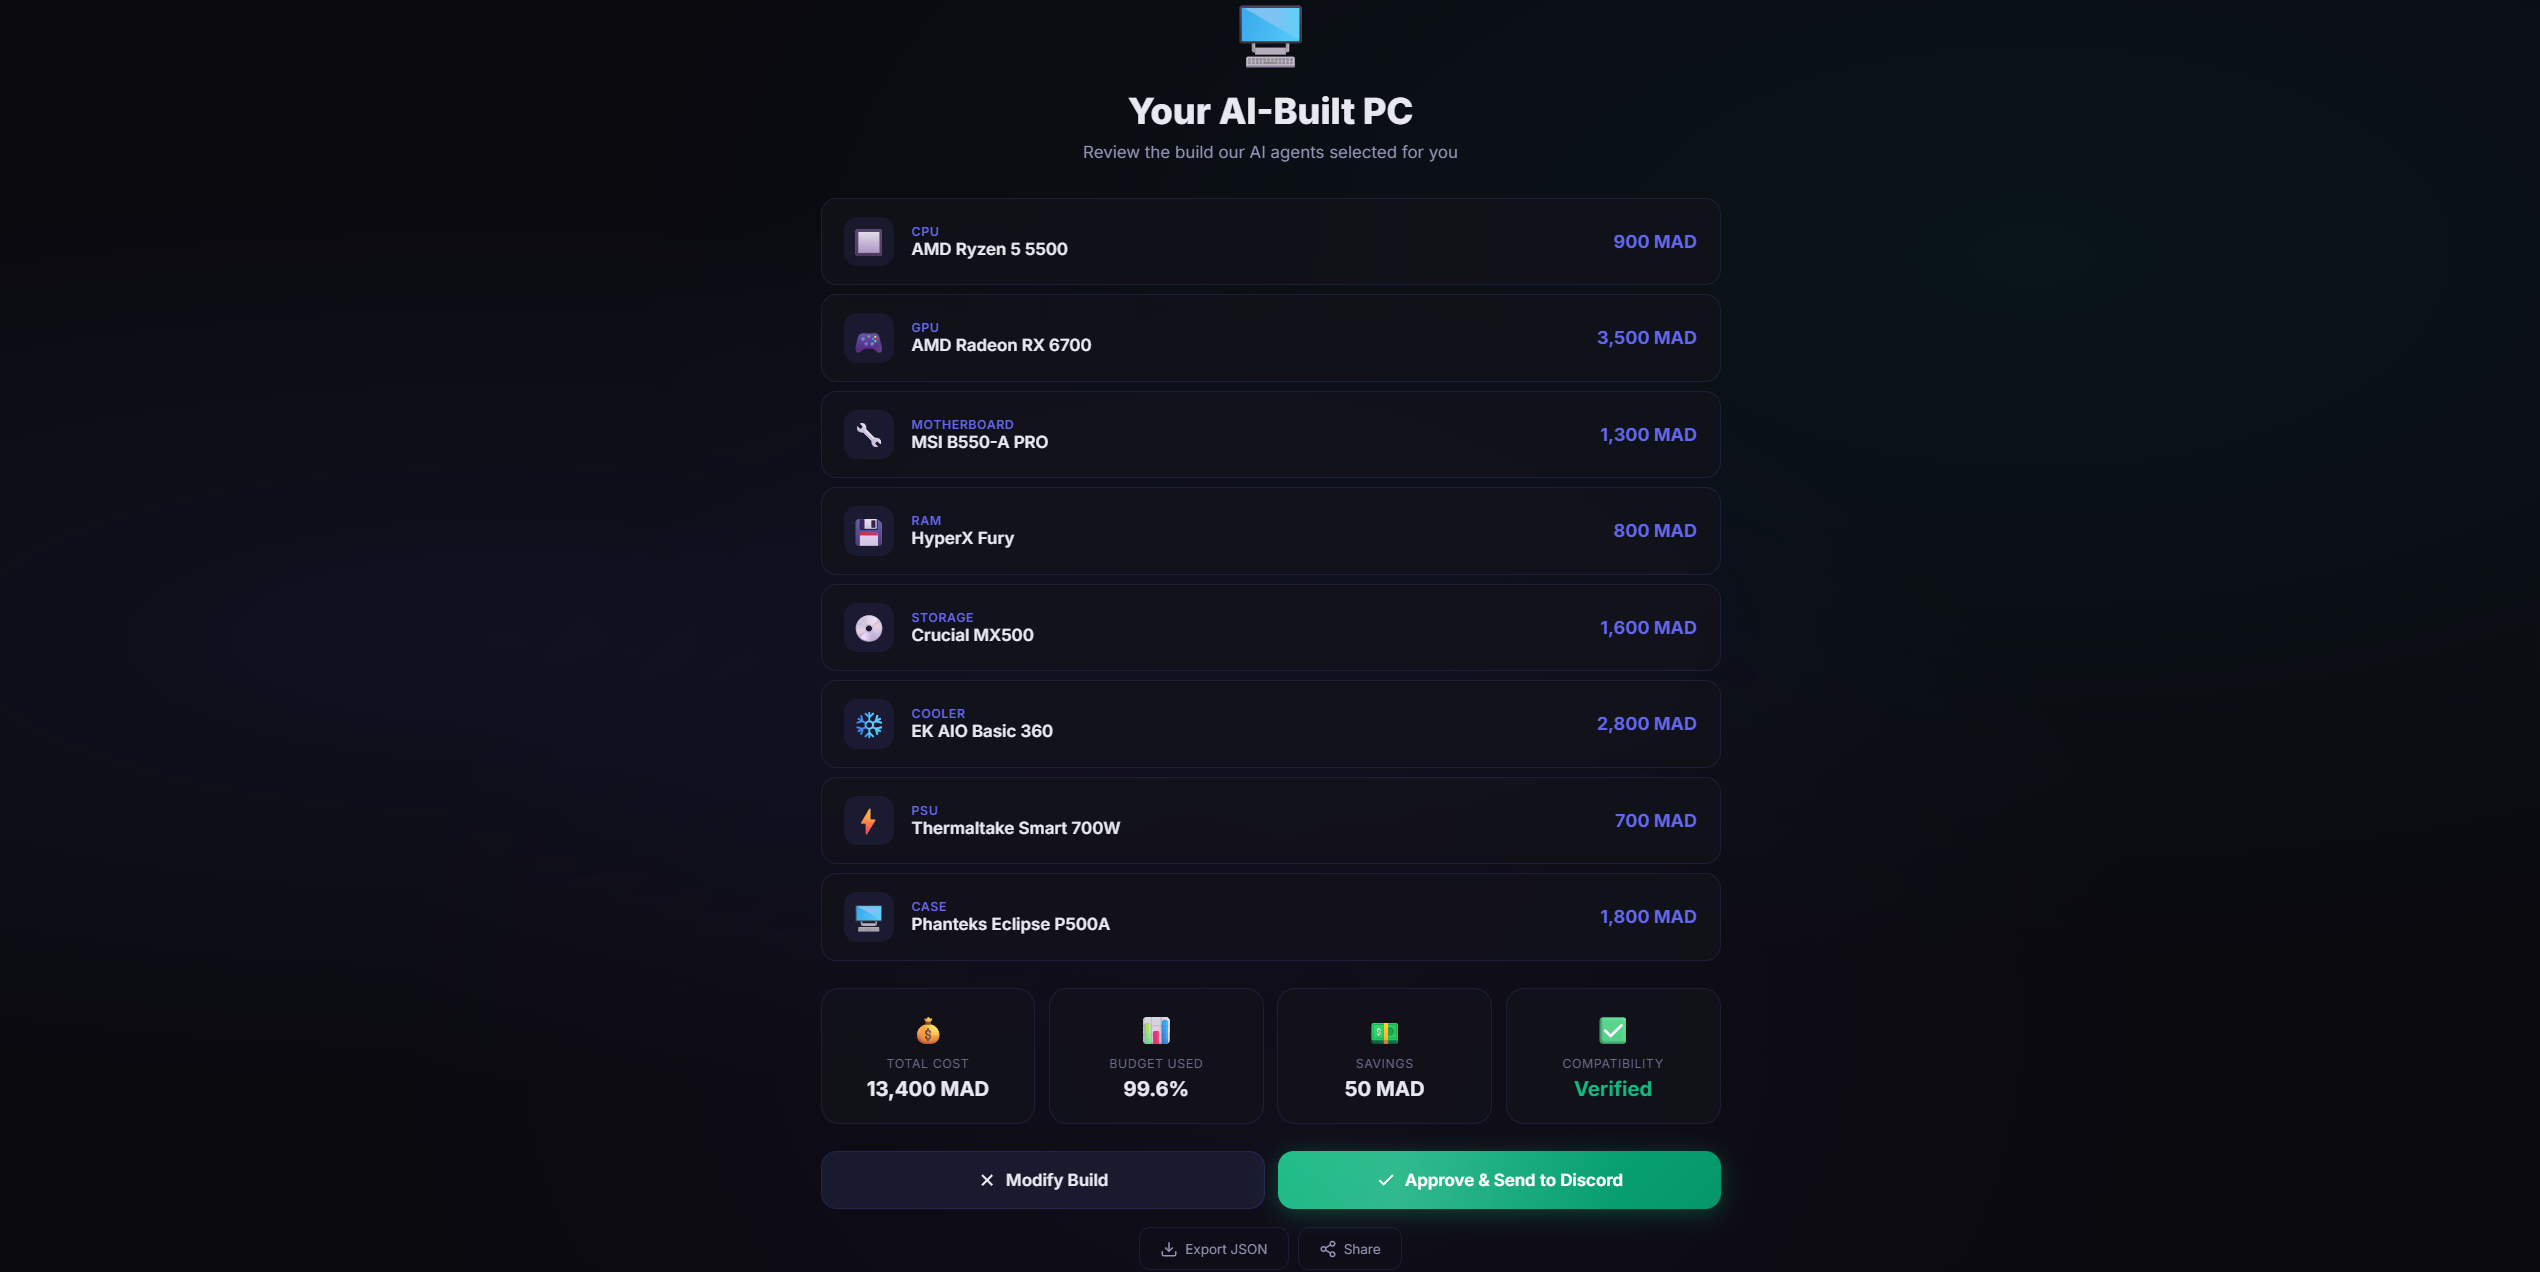
\includegraphics[width=0.85\textwidth]{summary.png}
\caption{\'Ecran r\'ecapitulatif : 8 composants s\'electionn\'es par l'IA avec co\^ut total et actions Approuver/Modifier}
\label{fig:summary}
\end{figure}

\begin{figure}[H]
\centering
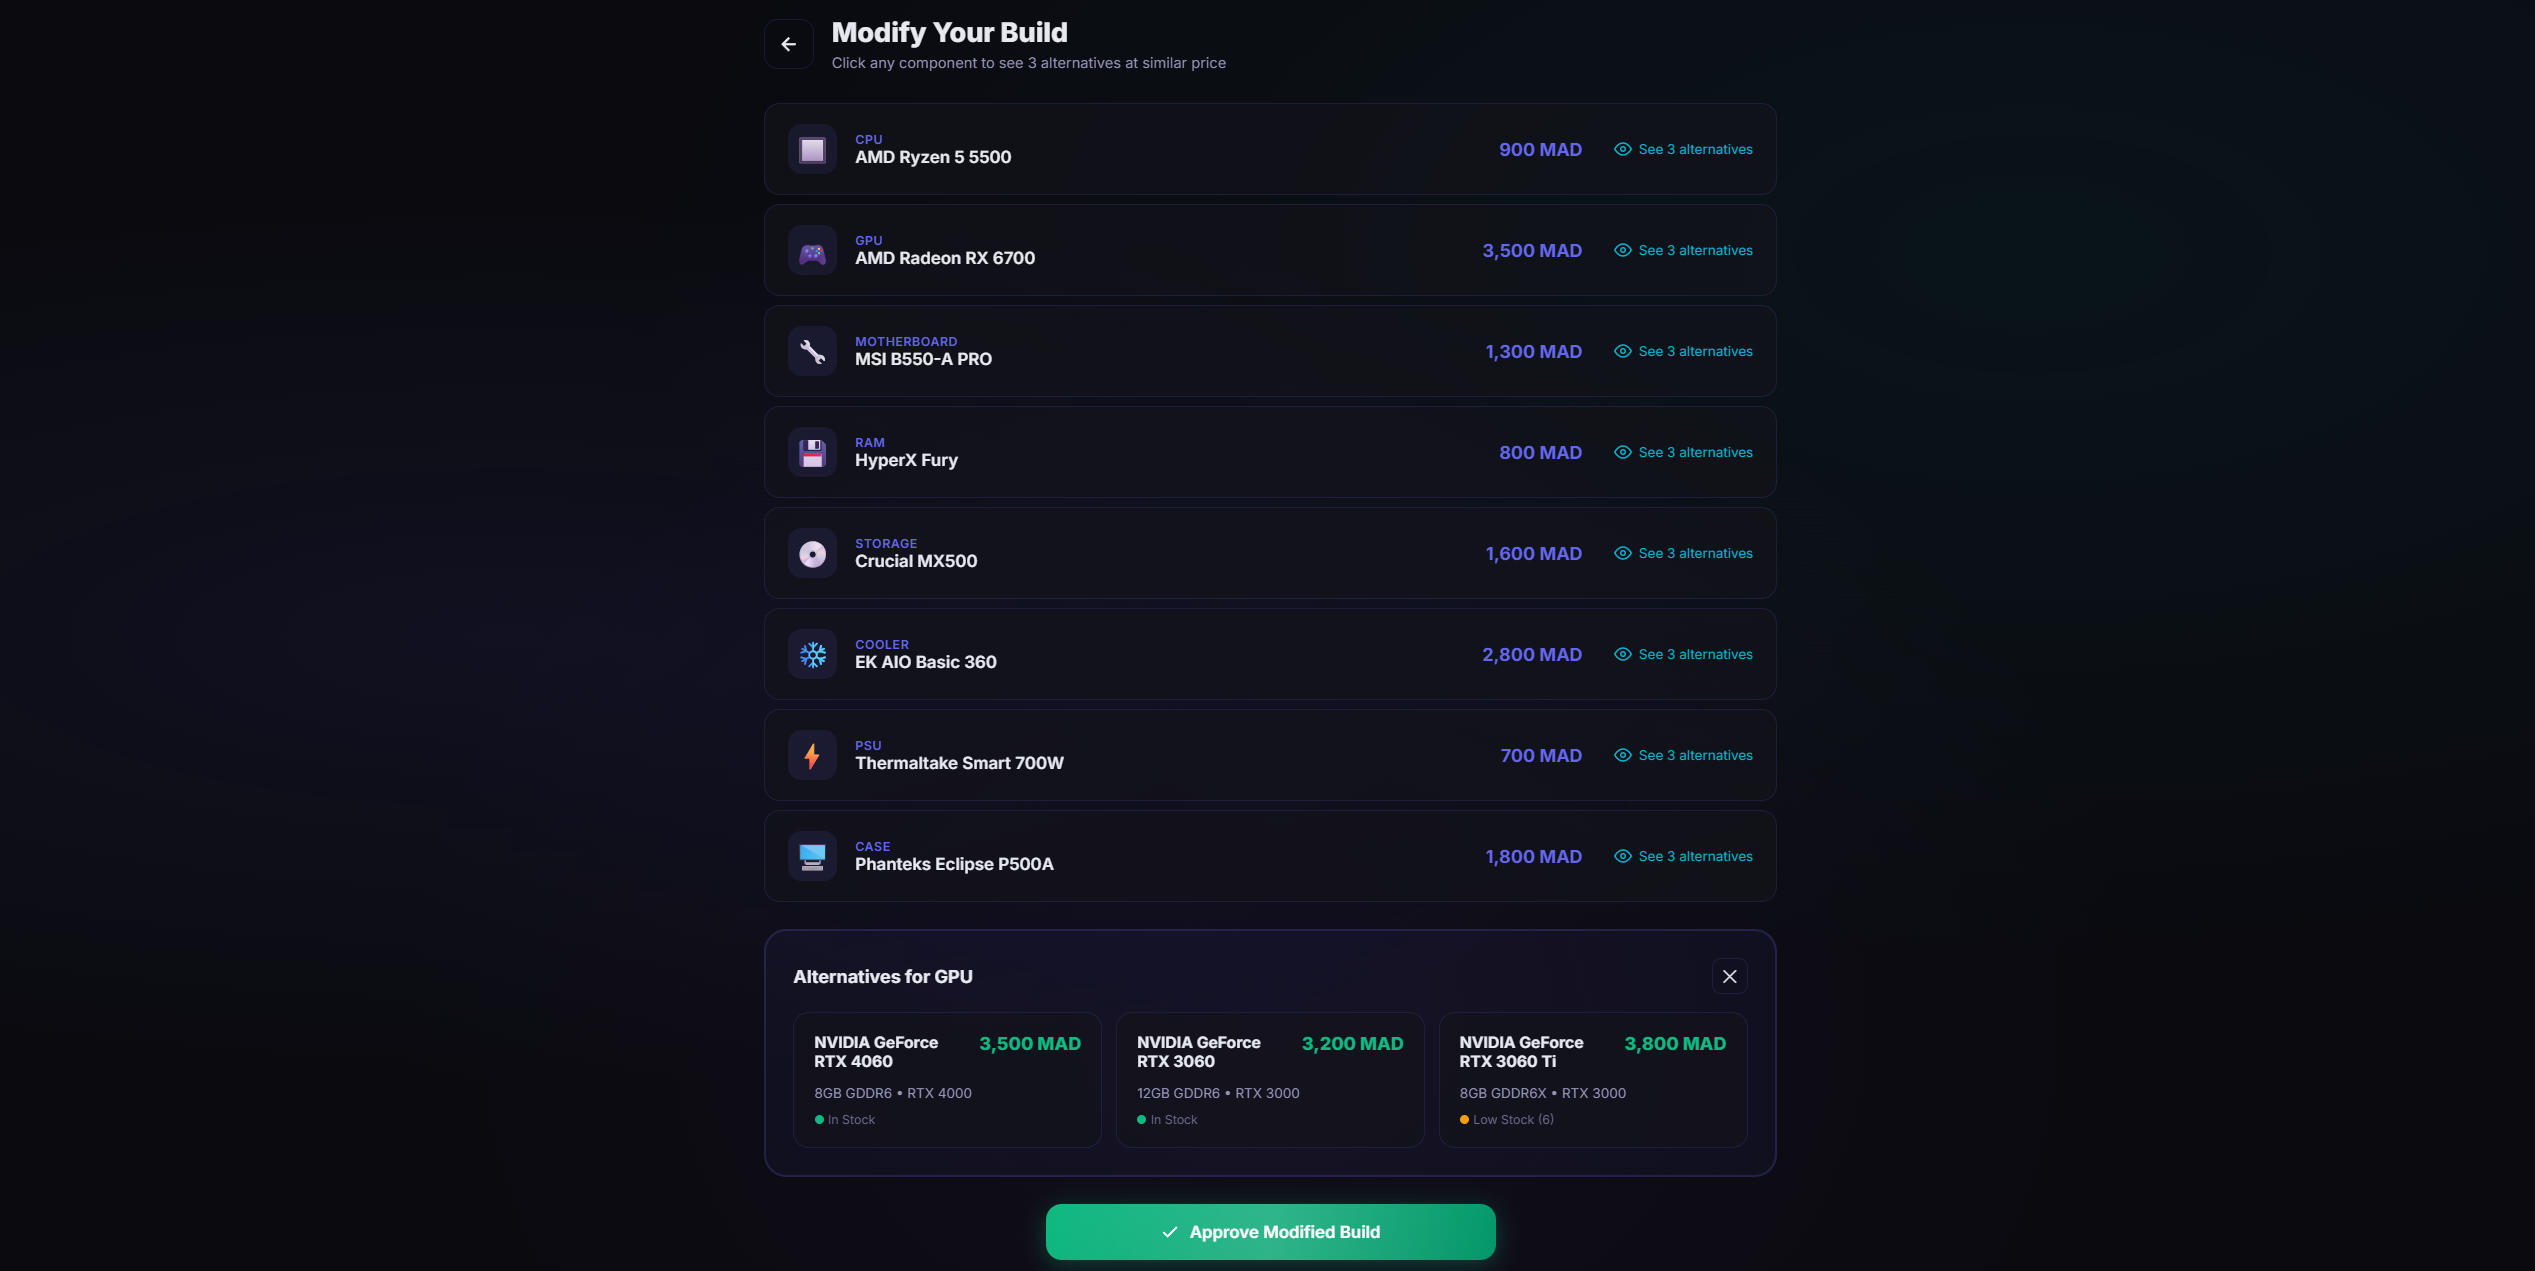
\includegraphics[width=0.85\textwidth]{modify.png}
\caption{\'Ecran de modification : chaque composant propose 3 alternatives compatibles au prix le plus proche}
\label{fig:modify}
\end{figure}

\begin{figure}[H]
\centering

\includegraphics[width=0.85\textwidth]{result.png}
\caption{\'Ecran de confirmation : build approuv\'e, inventaire mis \`a jour et notification Discord envoy\'ee}
\label{fig:result}
\end{figure}

\begin{figure}[H]
\centering
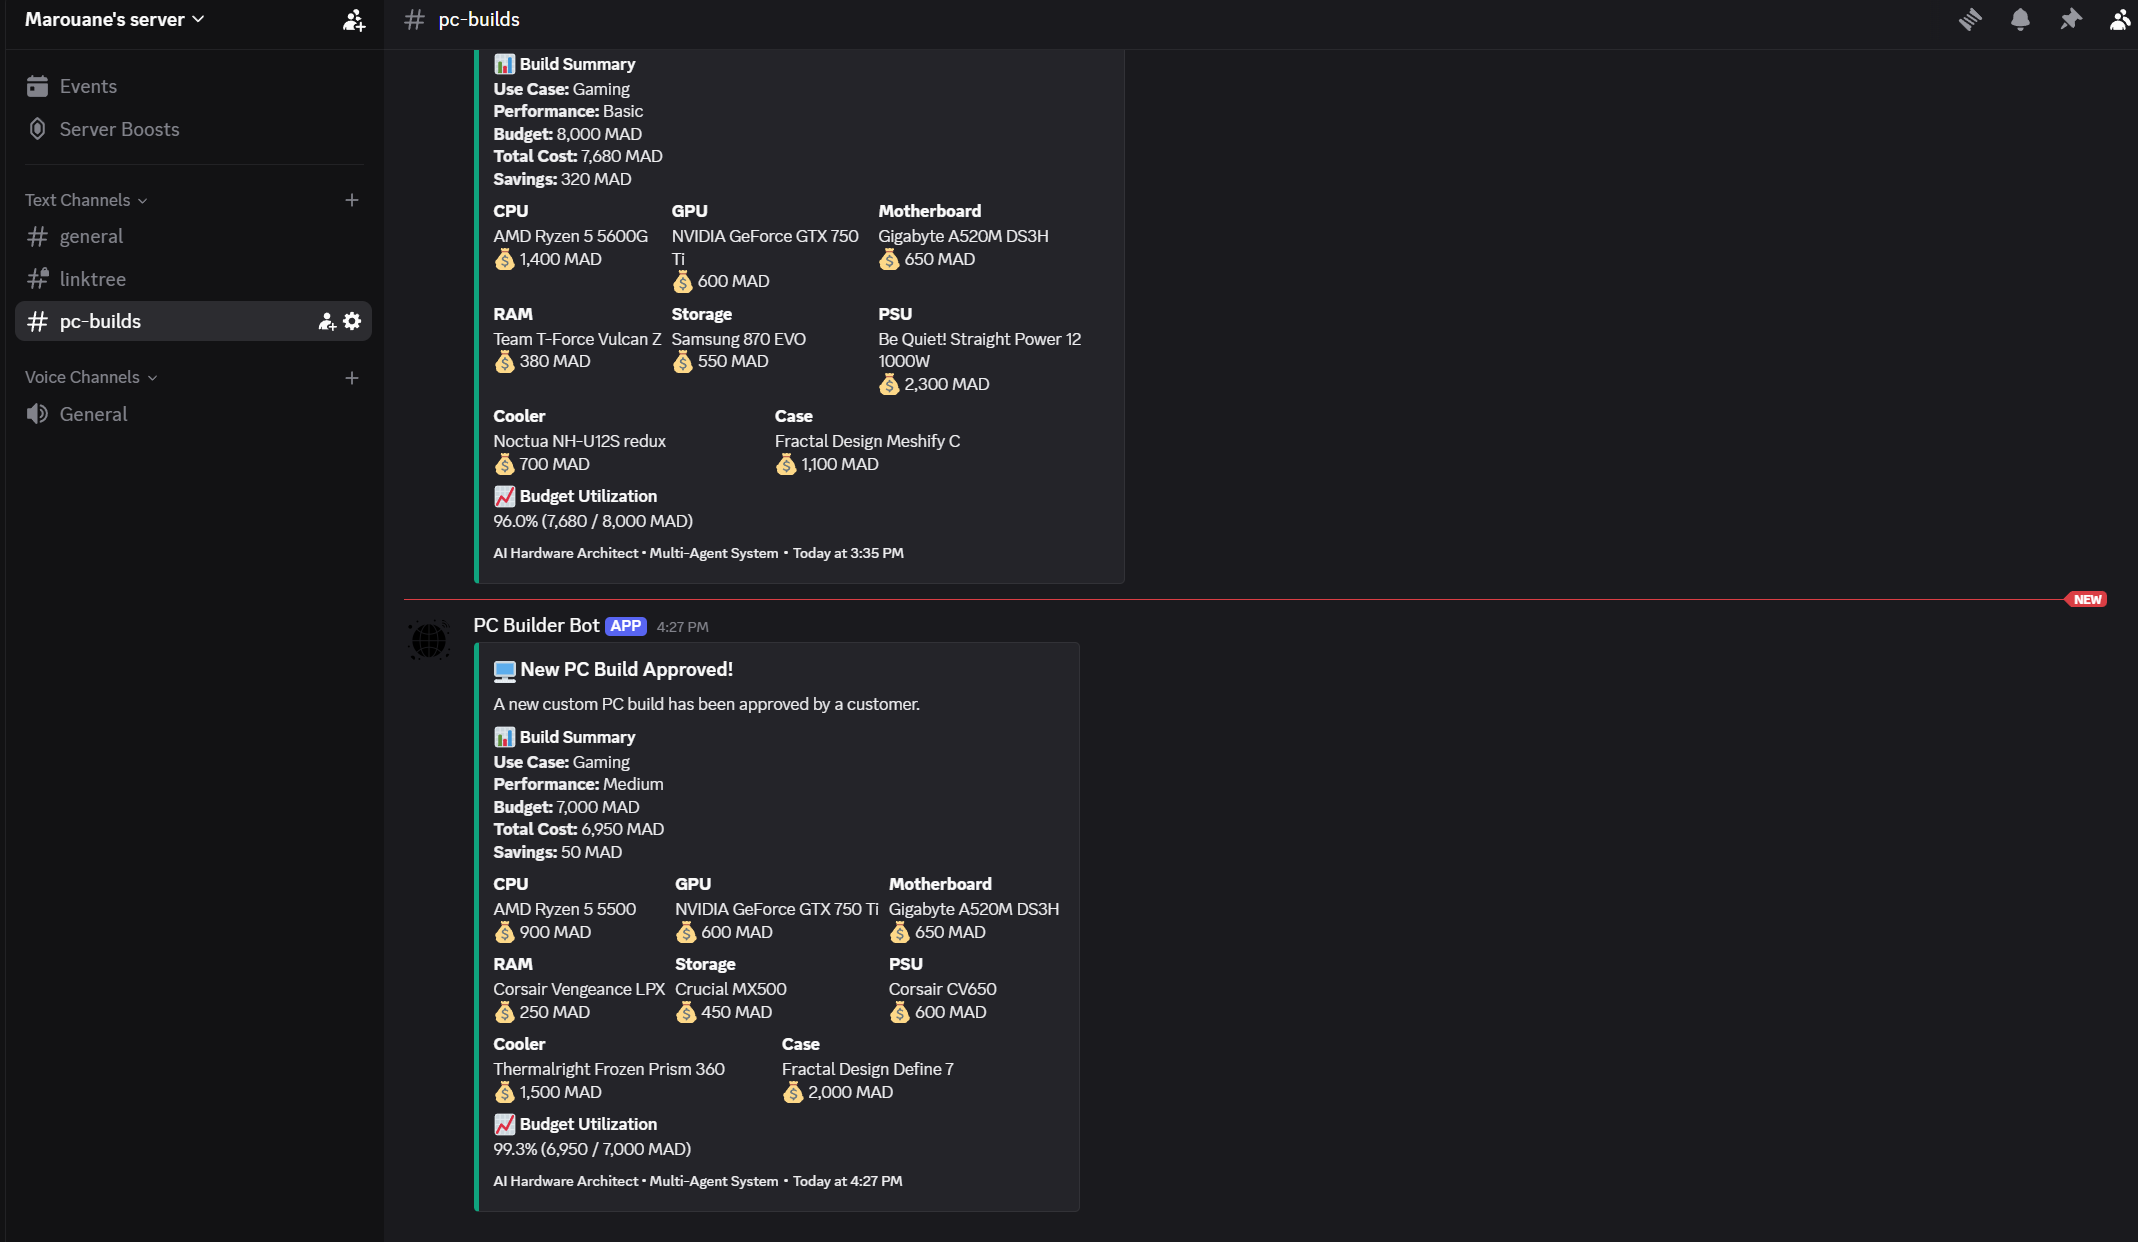
\includegraphics[width=0.85\textwidth]{discord.png}
\caption{Notification Discord : message automatique envoy\'e au canal d'\'equipe avec le d\'etail complet du build approuv\'e}
\label{fig:discord}
\end{figure}

\subsection{Int\'egration Discord et Gestion d'Inventaire}
Lorsque l'utilisateur approuve un build :
\begin{itemize}
    \item Le stock de chaque composant s\'electionn\'e est d\'ecr\'ement\'e automatiquement dans les fichiers CSV via le module \texttt{inventory\_manager.py}.
    \item Un message format\'e contenant le d\'etail complet du build est envoy\'e au canal Discord de l'\'equipe via un Webhook.
    \item L'historique de la d\'ecision est persist\'e dans la base MySQL pour audit.
\end{itemize}

\subsection{Architecture Modulaire du Human-in-the-Loop}
Le syst\`eme de validation humaine a \'et\'e enti\`erement refactoris\'e en une architecture modulaire comprenant trois composants principaux.

\subsubsection{Gestionnaire d'Approbation (ApprovalManager)}
Classe centrale g\'erant le cycle de vie des demandes d'approbation :
\begin{itemize}
    \item \textbf{Cr\'eation de requ\^etes :} G\'en\'eration d'identifiants uniques et horodatage
    \item \textbf{Validation de s\'ecurit\'e :} V\'erification automatique des configurations
    \item \textbf{Traitement des d\'ecisions :} Gestion des approbations/rejets avec feedback
    \item \textbf{Historique persistant :} Sauvegarde et export des d\'ecisions pour audit
\end{itemize}

\subsubsection{Interface Utilisateur Modulaire (HumanApprovalUI)}
Composants Flask/SocketIO sp\'ecialis\'es pour l'interaction humaine :
\begin{itemize}
    \item Interface d'approbation avec boutons contextuels
    \item Comparaison requ\^ete/build c\^ote-\`a-c\^ote
    \item Collecte de feedback avec zone de texte
    \item Statistiques en temps r\'eel et historique
\end{itemize}

\subsubsection{Int\'egration Workflow (HumanLoopWorkflow)}
Pont entre le syst\`eme d'approbation et LangGraph :
\begin{itemize}
    \item G\'en\'eration automatique de n\oe uds LangGraph
    \item Synchronisation entre l'\'etat workflow et les requ\^etes
    \item Nettoyage automatique des requ\^etes expir\'ees
    \item Sauvegarde et restauration de l'\'etat workflow
\end{itemize}

\subsection{Impl\'ementation Technique}

\begin{lstlisting}[caption={Int\'egration modulaire du Human-in-the-Loop}]
# Initialisation du systeme modulaire
from human_loop import (
    approval_manager, 
    create_approval_ui, 
    initialize_workflow_integration
)

# Configuration de l'integration workflow
workflow_integration = initialize_workflow_integration(
    approval_manager
)
approval_ui = create_approval_ui(approval_manager)

# Creation du noeud d'approbation pour LangGraph
human_approval_node = workflow_integration.create_human_approval_node()

# Integration dans le workflow
workflow.add_node("human_approval", human_approval_node)
\end{lstlisting}

\subsection{Fonctionnalit\'es Avanc\'ees}

\subsubsection{Validation Automatique de S\'ecurit\'e}
Le syst\`eme effectue des v\'erifications automatiques :
\begin{itemize}
    \item Validation budg\'etaire avec tol\'erance de 10 pourcent
    \item Contr\^ole de coh\'erence des composants essentiels
    \item V\'erification de format du devis g\'en\'er\'e
    \item D\'etection d'anomalies dans les prix
\end{itemize}

\subsubsection{Persistance et Audit}
\begin{itemize}
    \item Export JSON avec sauvegarde automatique des d\'ecisions
    \item Statistiques d'approbation (taux, temps de d\'ecision moyen)
    \item Tra\c{c}abilit\'e compl\`ete avec historique et feedback
    \item Nettoyage automatique des requ\^etes expir\'ees
\end{itemize}

\section{Structure du Projet}

Le projet est organis\'e de mani\`ere modulaire :

\textbf{Dossier agents/} : Syst\`eme multi-agent
\begin{itemize}
    \item graph.py : Orchestration LangGraph
    \item nodes.py : Impl\'ementations des agents
\end{itemize}

\textbf{Dossier human\_loop/} : Syst\`eme Human-in-the-Loop
\begin{itemize}
    \item approval\_manager.py : Gestionnaire d'approbation
    \item ui\_components.py : Interface utilisateur
    \item workflow\_integration.py : Int\'egration workflow
\end{itemize}

\textbf{Dossier evaluation/} : Framework d'\'evaluation
\begin{itemize}
    \item prompt\_evaluation.py : Tests de performance
    \item ab\_testing.py : Tests A/B
    \item metrics\_dashboard.py : Dashboard de monitoring
\end{itemize}

\textbf{Dossier rag/} : Syst\`eme RAG
\begin{itemize}
    \item ingest.py : Ingestion des donn\'ees
    \item chroma\_db/ : Base vectorielle
\end{itemize}

\textbf{Dossier data/} : Bases de donn\'ees composants (8 fichiers CSV : cpus, gpus, motherboards, ram, storage, coolers, psus, cases)

\textbf{Dossier database/} : Gestionnaire MySQL (db\_manager.py) pour la persistance

\textbf{Fichier app.py} : Serveur Flask/Socket.IO avec APIs REST (/api/components/recommend, /api/components/alternatives) et handlers Socket.IO

\textbf{Fichier inventory\_manager.py} : Gestion du stock (d\'ecr\'ementation automatique apr\`es approbation)

\section{Conclusion et Perspectives}

\subsection{R\'ealisations Accomplies}
Ce projet d\'emontre la puissance d'une architecture multi-agent modulaire et orchestr\'ee. Nous avons r\'eussi \`a impl\'ementer tous les composants requis :

\begin{itemize}
    \item \textbf{Orchestration Multi-Agent :} Architecture LangGraph avec agents sp\'ecialis\'es et modulaires
    \item \textbf{RAG Agentique :} Syst\`eme de r\'ecup\'eration augment\'ee avec base vectorielle ChromaDB
    \item \textbf{Human-in-the-Loop Avanc\'e :} Syst\`eme complet de validation avec interface modulaire
    \item \textbf{Interface Web Interactive :} Application Flask/Socket.IO avec wizard interactif, visualisation du pipeline multi-agent en temps r\'eel, et m\'ecanisme de modification avec alternatives
    \item \textbf{Evaluation des Prompts :} Framework complet avec tests A/B et optimisation
\end{itemize}

\subsection{Innovations Techniques}
\begin{itemize}
    \item \textbf{Architecture Modulaire :} S\'eparation claire des responsabilit\'es en modules ind\'ependants
    \item \textbf{Syst\`eme d'Approbation Sophistiqu\'e :} Gestion d'\'etat persistant et validation automatique
    \item \textbf{Interface Wizard :} Exp\'erience utilisateur guid\'ee avec alternatives intelligentes (3 composants au prix le plus proche avec filtrage de compatibilit\'e)
    \item \textbf{Optimisation Bas\'ee sur les Donn\'ees :} Tests A/B avec am\'elioration de 41 pourcent
    \item \textbf{Int\'egration Discord :} Notification automatique de l'\'equipe avec Webhook
    \item \textbf{Robustesse Op\'erationnelle :} M\'ecanismes de fallback Pandas et gestion d'erreurs
\end{itemize}

\subsection{Impact Acad\'emique}
Le syst\`eme illustre l'application pratique des concepts th\'eoriques du cours SMA et IAD :
\begin{itemize}
    \item Coordination Multi-Agent avec orchestration s\'equentielle
    \item Interaction Homme-Machine avec validation humaine
    \item Optimisation Algorithmique par \'evaluation empirique
    \item Ing\'enierie Logicielle avec architecture maintenable
\end{itemize}

\subsection{Perspectives d'Am\'elioration}
\begin{itemize}
    \item Agent V\'erificateur Ind\'ependant pour simulation de benchmarks
    \item Optimisation Multi-Objectifs avec algorithmes g\'en\'etiques
    \item Apprentissage Adaptatif bas\'e sur l'historique des approbations
    \item Int\'egration E-commerce avec APIs de fournisseurs
    \item Syst\`eme de Recommandation avec ML pour suggestions personnalis\'ees
\end{itemize}

\subsection{Validation Exp\'erimentale}
Les tests A/B ont d\'emontr\'e l'efficacit\'e de notre approche avec des am\'eliorations mesurables de 41 pourcent entre les strat\'egies de prompts, validant scientifiquement notre m\'ethodologie d'optimisation.

\vspace{1cm}
\textbf{Lien vers le code source (GitHub) :} \\
\url{https://github.com/marouane-m7b/ENSET_PFM_Agent_Building_PC}

\end{document}